\documentclass{beamer}
\usepackage{beamerthemesplit}
\usepackage{graphics}
\logo{
\includegraphics[height=1cm]{psi_logo_white.png}}
\usetheme{Pittsburgh}
\usecolortheme{dove}
\beamertemplatenavigationsymbolsempty
\setbeamertemplate{footline}[frame number]
\definecolor{myback}{RGB}{175,238,238}
\setbeamercolor{structure}{bg=myback}
\usepackage[T1]{fontenc}
\newcommand{\changefont}[3] {
 \fontfamily{#1} \fontseries{#2} \fontshape{#3} \selectfont}

\title{NeXus Application Definitions Tutorial}
\author{Mark K\"onnecke }
\institute{Paul Scherrer Institute\\Switzerland }
\date{\today} 

\begin{document}

\begin{frame}
\titlepage
\end{frame}

\begin{frame}
\frametitle{Your Task:}
\begin{itemize}
\item Develop an application definition for WONI at INIS
\item WONI = WOnderful New Instrument
\item INIS = INsanely Intense Source
\end{itemize}
\end{frame}


\begin{frame} \frametitle{WONI Design}
\begin{figure}[!ht]
\resizebox{7cm}{5cm}{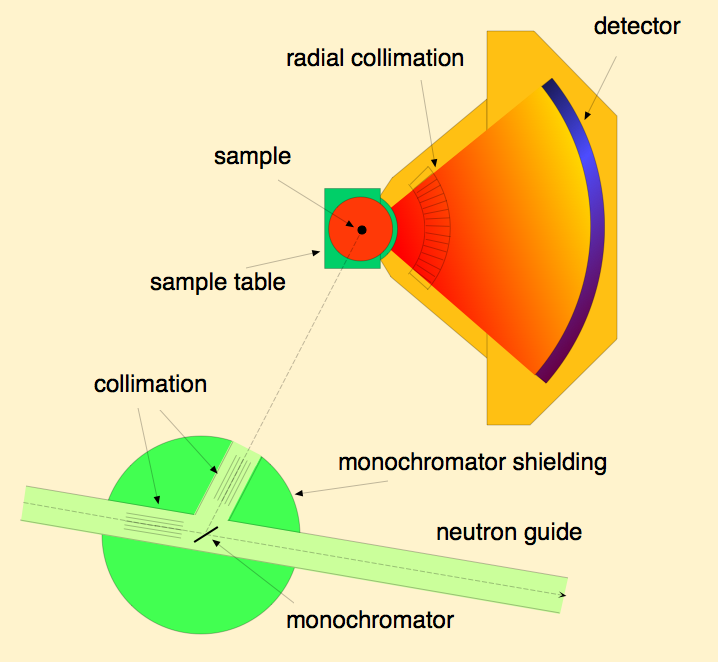
\includegraphics[width=0.85\textwidth]{dmc.png}}\end{figure}
\end{frame}

\begin{frame} \frametitle{WONI Plot}
\begin{figure}[!ht]
\resizebox{7cm}{5cm}{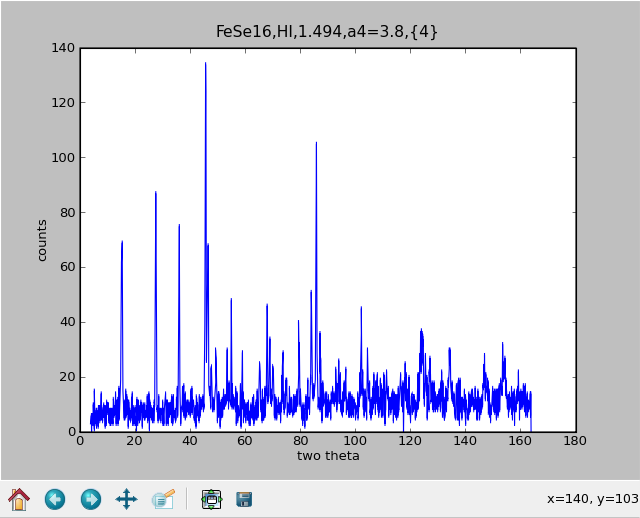
\includegraphics[width=0.85\textwidth]{powderimage.png}}\end{figure}
\end{frame}


\begin{frame}
\frametitle{What You Need}
\begin{itemize}
\item A copy of the current NeXus base class definitions
\item A XML editor 
\end{itemize}
\end{frame}


\begin{frame}
\frametitle{Four Steps}
\begin{enumerate}
\item {\color{blue} Think!} what ought to go into the file
\item {\color{blue}Map }this into the NeXus file structure
\item {\color{blue} Cast} this mapping into a NXDL file
\item {\color{blue} Standardize} your application definition together with the NIAC
\end{enumerate}
\end{frame}


\begin{frame}
\frametitle{Think!}
\begin{itemize}
\item What has to go into the file?
\item Minimum data necessary for common usage scenarios
\item Haggle it out with your community
\item Coverage ratio: $> 80$ \% of use cases
\end{itemize}
\end{frame}

\begin{frame}
\frametitle{Think! for WONI}
\begin{itemize}
\item Common usage is Rietveld analysis or profile analysis
\item Data required:
\begin{itemize}
\item Title
\item Sample name
\item Wavelength
\item Counts versus two\_theta
\item Monitor, for normalisation
\end{itemize}
\end{itemize}
\end{frame}

\begin{frame}
\frametitle{Map to NeXus}
\begin{itemize}
\item Consider into which NeXus group an item might belong
\item Look in the base class for a suitable data field
\item Link the data items required for the default plot into NXdata
\end{itemize}
\end{frame}

\begin{frame} \frametitle{Mappings for WONI}
\begin{tabbing}
\hspace*{1cm} \= \hspace*{1cm} \= \hspace*{1cm} \= \hspace*{1cm} \= \kill
\uncover<1-> {
entry:NXentry \\
\>title\\
\>definition\\
}
\uncover<2->{
 \>sample:NXsample \\
 \> \> name \\
}
\uncover<3->{
 \>instrument:NXinstrument\\
 \> \>monochromator:NXmonochromator\\
 \> \> \>wavelength\\
}
\uncover<4->{
 \> \> detector:NXdetector \\
 \> \> \>data[ndet], signal=1 (1)\\
 \> \> \>polar\_angle[ndet], axis=1 (2)\\
}
\uncover<5->{
\>control:NXmonitor\\
\> \>data\\
}
\uncover<6-> {
\>data:NXdata\\
\> \>link to (1)\\
\> \>link to (2)\\
}
 \end{tabbing}
\end{frame}

\begin{frame}[fragile]
\frametitle{Casting into NXDL: groups}
\begin{semiverbatim}
<group type="NXsource" name=''source''>

</group>
\end{semiverbatim}
\end{frame}

\begin{frame}[fragile]
\frametitle{Casting into NXDL: fields}
\begin{semiverbatim}
<field name="data" type="NX_INT" signal="1">
     <doc>
       Some blabla
     </doc>
     <dimensions size="3">
         <dim index="1" value="np" />
         <dim index="2" value="number of x pixels" />
         <dim index="3" value="number of y pixels" />
     </dimensions>
     <attribute name="signal" type="NX_CHAR">
         <enumeration>
            <item value="1" />
          </enumeration>
      </attribute>
</field>
\end{semiverbatim}
\end{frame}

\begin{frame} \frametitle{Editing in Eclipse}
\begin{itemize}
\item There is a XML schema for NXDL, the editor helps you! 
\end{itemize}
\end{frame}

\begin{frame}
\frametitle{Standardisation}
\begin{itemize}
\item Forward you application defintion to the NIAC for review
\item Correct you definition according to NIAC comments, if any
\item Cure and use the definition for a year, data should be written and analysed in this year
\item After a final review, this is the standard for that application. Period. 
\end{itemize}
\end{frame}

\begin{frame}
\frametitle{From an application definition to a real NeXus file}
\begin{itemize}
\item<1->The structure defined by the application definition is the minimum
\item<2->Practical files strive to capture much more
\uncover<3->{
\item Suggested procedure:
\begin{itemize}
\item Look at each of your instruments components and the matching NeXus base class
\item Add whatever you feel like adding or the instrument scientists wants to have
\item Add whatever management wants to have (may be not in a NeXus group)
\end{itemize}
}
\item<4-> Remember: {\color{red}Adding more fields does not break application definition compliance!} 
\end{itemize}
\end{frame}

\begin{frame} \frametitle{What about ONOKI?}
\begin{itemize}
\item<1->ONOKI: ONe Of a Kind Instrument
\item<2->{\color{blue}Think!} what you want to store
\item<3->{\color{blue}Map} the list into the appropriate NeXus base classes. It helps to 
 look at each of the components ONOKI is assembled from and to decide what you wish 
 to store for each of them. 
\item<4->The next one to copy ONOKI is well advised to copy what you did NeXus file wise, 
 otherwise she will not be able to reuse your software!
\end{itemize}
\end{frame}

\begin{frame}
\frametitle{Validation}
\begin{itemize}
\item Not quite ready yet
\item nxvalidate  nexusfile.hdf
\end{itemize}
\end{frame}

\end{document}


\begin{frame}
\frametitle{}
\begin{itemize}
\item
\end{itemize}
\end{frame}


\begin{frame} \frametitle{Using Tabbing for Hierarchy}
\begin{tabbing}
\hspace*{1cm} \= \hspace*{1cm} \= \hspace*{1cm} \= \hspace*{1cm} \= \kill
entry:NXentry \\
 \>sample:NXsample \\
 \> \> rotation\_angle[NP], axis=1 (1) \\
\\
 \>instrument:NXinstrument\\
 \> \> detector:NXdetector \\
 \> \> \>data[NP], signal=1 (2)\\
 \>data:NXdata\\
 \> \> link to (1)\\
 \> \> link to (2)\\
\end{tabbing}
\end{frame}

